\documentclass[a4paper, 11pt]{article}
\usepackage{geometry}
\geometry{letterpaper, margin=1in}
\usepackage{amsmath}
\usepackage{amssymb}  
\usepackage{amsthm}
\usepackage{ulem} 
\usepackage{graphicx}
\usepackage{enumitem} % use for making lettered list 
\usepackage{bbm} % use for making the 1 identity operator EX: \mathbbm{1}
\usepackage{subfig} 
\graphicspath{ {images/} }

% format to allow bolded theorems, corollaries, etc... 
\newtheorem*{theorem}{Theorem}
\newtheorem*{corollary}{Corollary}
\newtheorem*{lemma}{Lemma}
\newtheorem*{definition}{Definition}





\begin{document}
%Header-Make sure you update this information!!!!
\noindent
\large\textbf{Global Gauss-Bonnet} \hfill \textbf{John Waczak} \\
\normalsize MTH 435 \hfill  Date: \today \\
Dr. Christine Escher \\
\par\noindent\rule{\textwidth}{0.4pt}	
	

\subsection*{Tapp 6.12}
	\textit{A soccer ball is constructed from 12 pentagonal faces and 20 hexagonal faces. Consider this generalized triangulation of $S^2$. Calculate $V$, $E$, and $F$ and use this to again show that $\chi(S^2)=2$. }\\

	

	\noindent The following images show the entire soccer ball as well as one way to put the polygons together in order to make one hemisphere of the triangulation. Imagine allowing the rigid edges to curve so that the cuts in (b) can be joined to close the surface. 
		\begin{figure}[!hbt]
			\centering
			\subfloat[soccer ball]
				{
					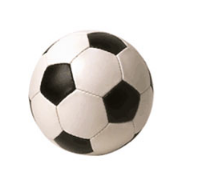
\includegraphics[width=0.3\columnwidth]{soccerBall}
				}
			\quad
			\subfloat[hemisphere triangulation]
				{
					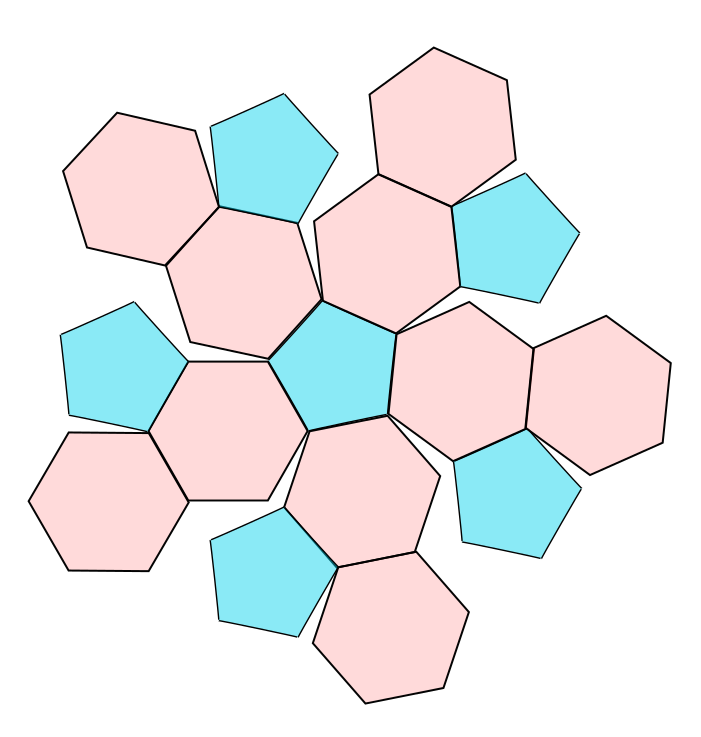
\includegraphics[width=0.35\columnwidth]{soccerBallHemisphere}	
				}
			\caption{The soccer ball triangulation of $S^2$} 
			\label{fig:soccerBall}
		\end{figure}
	
		\begin{proof}
			Observe that every vertex in  this triangulation is shared by 3 faces and every edge is shared by two faces. Thus we have 
				\begin{equation*}
					\begin{cases}
						V &= \frac{(12\cdot 5)+(20\cdot 6)}{3} = \frac{180}{3} =60 \\
						E &=  \frac{(12\cdot 5)+(20\cdot 6)}{2} = \frac{180}{2} = 90 \\ 
						F &= (12\cdot 3)+(20\cdot 6) = 32 \\ 
					\end{cases}
				\end{equation*}
			Thus the Euler characteristic for this triangulation $T$ is
				\begin{equation*}
					\chi(T) = 30-90+32 = 2 = \chi(S^2) 
				\end{equation*}
		\end{proof}

\subsection*{Tapp 6.13}
	\textit{The following figure shows a torus with a rectangular triangulation. Explain why $F = V = \frac{E}{2}$ and use this to again verify that the Euler characteristic of the torus is 0. }\\
	
	\begin{figure}[!hbt]
		\centering
		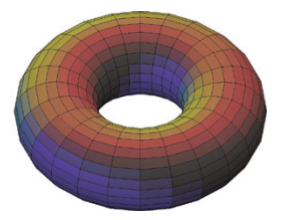
\includegraphics[width=0.45\columnwidth]{torusWithRectangulation}
		\caption{A torus with a rectangular triangulation} 
		\label{fig:torus} 
	\end{figure}
	
	\noindent We will use this figure to verify the above statement. \\ 
	
	\begin{proof}
		From figure \ref{fig:torus} we can observe that every vertex is shared by 4 faces. Thus if we count up all the faces \textit{without} double counting we see that there are $V=F$ vertices. It is also clear that every edge is shared by two faces and each rectangular face has 4 edges. Thus the total number of edges without double counting is given by $E = \frac{4F}{2} = 2F$ which implies that $F = \frac{E}{2}$. Using this information, we can solve for the Euler characteristic in terms of F. 
			\begin{equation*}
				\chi(T^2) = V-E+F = F-2F+F = 0
			\end{equation*}
		Thus once again we have found that $\chi(T^2) =0$ as we expect. 
	\end{proof}
	
	
	
	
	
\subsection*{Problem 2}
	\textit{Find the total Gaussian curvature of \begin{enumerate}[label=\alph*]
			\item An ellipsoid 
			\item $S = \{(x,y,z)\in\mathbb{R}: x^2+y^{10}+z^6=1\}$
		\end{enumerate}}
	
	\begin{proof}[(a) Ellipsoid]
		The general implicit definition for an ellipsoid is
			 \begin{equation*}
				 E = \{(x,y,z)\in\mathbb{R}:\frac{x^2}{a^2}+\frac{y^2}{b^2}+\frac{z^2}{c^2} = 1\}
			 \end{equation*}

			\begin{figure}[!hbt]
				\centering
				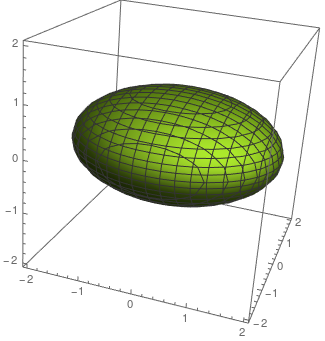
\includegraphics[width=0.35\columnwidth]{ellipsoid}
			\end{figure}
			
		\noindent We can easily construct a homeomorphism to the sphere $S^2 = \{(x,y,z)\in\mathbb{R}:x^2+y^2+z^2=1\}$ via the following function $\phi:S^2\to E$ which maps such that
			\begin{equation*}
				\phi(x,y,z) = \Big(\frac{x}{a}, \frac{y}{b}, \frac{z}{c}\Big)
			\end{equation*}
		This function is certainly a bijection as it has inverse
			\begin{equation*}
				\phi^{-1}(x,y,z) = (ax, by, cz)
			\end{equation*}
		Both $\phi, \phi^{-1}$ are continuous as each function only scales by the constants $x,y,z\in\mathbb{R}$ with $a,b,c\neq 0$. Thus $E$ is homeomorphic to the sphere. Because the sphere is a compact surface, the image of $S^2$ under $\phi$, i.e. $E$ is a compact surface. Then because $E \cong_{\text{homeo}} S^2$, these surfaces must have the same Euler characteristic i.e. $\chi(E) = \chi(S^2) = 2$. Therefore we conclude that
			\begin{equation*}
				\iint K d\sigma = 2\pi\chi(E) = 2\pi\chi(S^2)=4\pi 
			\end{equation*}
	\end{proof}
	
	
	\begin{proof}[(b) S]
		For this next surface, we will follow the same proof structure. \\
		\begin{figure}[!hbt]
			\centering
			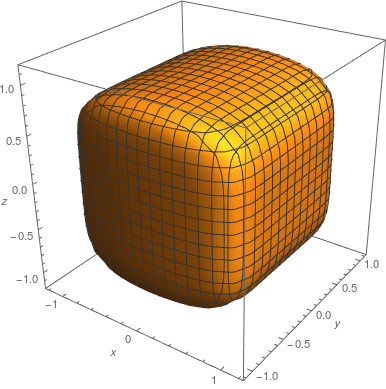
\includegraphics[width=0.35\columnwidth]{breadSurface}
		\end{figure}
	
	\noindent Consider the function $\psi(x,y,z) = (x, x^5, z^3)$. This function is certainly a bijection as odd polynomials have a domain of all of $\mathbb{R}$ (onto) and maintain sign i.e. $(-x)^{2n+1} = -(x^{2n+1}), n\in\mathbb{Z}^+$ (one to one). The inverse function is
		\begin{equation*}
			\psi^{-1}(x,y,z) = (x, y^{1/5}, z^{1/3})
		\end{equation*}
	which maps the surface $S$ back to the sphere $S^2$. Thus $\psi$ is a bijection. The functions ${x,x^3,x^5}$ are certainly continuous and it can be shown $x^{1/3}, x^{1/5}$ via an $\epsilon-\delta$ argument. Thus we have a homeomorphism between the sphere and $S$. Because the sphere is a compact surface then the image of $S^2$ under the homeomorphism is also compact, that is, $S$ is compact. Then the same argument as part (a), because $S, S^2$ must share the same Euler characteristic. Therefore, we have that:
		\begin{equation*}
			\iint K d\sigma = 2\pi\chi(S) = 2\pi\chi(S^2)=4\pi 
		\end{equation*}
		
	\end{proof}
	
	\noindent Intuitively this makes sense as looking at the graphs of both surfaces, each appears compact and we could almost trivially find their Euler characteristics to be $2$ using the same \textit{octant} triangulation we employed in class to determine $\chi(S^2)=2$. 

\subsection*{Problem 3}
	\textit{Prove that for a compact, connected, orientable regular surface in $\mathbb{R}^3$ that \begin{enumerate}[label=\alph*]
			\item $K>0\Rightarrow S$ is homeomorphic to a sphere 
			\item $K=0\Rightarrow S$ is homeomorphic to a torus
			\item $K<0\Rightarrow S$ is homeomorphic to a sphere with $g\geq 2$ handles. 
		\end{enumerate}}
	
	\begin{proof}[(a)]
		Let $S$ be a surface with above hypotheses satisfied and with $K>0$. Assume for contradiction that $S$ is \textit{not} homeomorphic to $S^2$. Then by \textit{Theorem 6.16}, it must be true that $\chi(S)\neq\chi(S^2) = 2$. Then again by applying \textit{Theorem 6.16} since $\chi(S)\neq 2$ it follows that $\chi(s)\leq 0$. Because S is compact, we can therefore write
			\begin{equation*}
				\iint K d\sigma = 2\pi\chi(S)
			\end{equation*}
		The right hand side must be non-positive by our previous argument which contradicts that assumption that $K>0$.  $(\rightarrow \leftarrow)$
	\end{proof}
	
	\begin{proof}[(b)]
		We will follow a similar procedure as in (a). Let $S$ be a surface satisfying the hypotheses and having $K=0$. Assume for contradiction that $S$ is \textit{not} homeomorphic to the torus. Then by application of \textit{Theorem 6.16} it follows that $\chi(S)=\neq\chi(T^2)=0$. This implies that there are two cases to consider: $\chi(S) = 2$ or $\chi(S) < 0$. \\ 
		
		\noindent For the first case, if $\chi(S) = 2$, we have that the compactness of $S$ implies
			\begin{align*}
				\iint K d\sigma = 2\pi\chi(S) = 4\phi
			\end{align*}
		This contradicts the assumption that $K$ is identically $0$. $(\rightarrow \leftarrow)$. \\ 
		
		\noindent For the second case, if $\chi(S)<0$ then we have that the compactness of S implies 
			\begin{equation*}
				\iint K d\sigma = 2\pi\chi(S) < 0
			\end{equation*}
		If $K$ is identically $0$ then there is no way that summing $K$ over the surface could result in a negative number. Again we have a contradiction. $(\rightarrow\leftarrow)$. Therefore, both cases lead to a contradiction which implies that if $K\equiv0$, the surface $S$ must be homeomorphic to the torus $T^2$ (even though we discussed in class that we cant have a compact surface with identically zero curvature sitting in $\mathbb{R}^3$).
		
		\begin{proof}[(c)]
			Let S be a surface satisfying the above hypotheses with $K<0$. Assume for contradiction that $S$ is \textit{not} homeomorphic to the sphere with $g\geq 2$ handles which I will denote $S_g^2$. Then by application of \textit{Theorem 6.16} we have that $\chi(S)\neq \chi(S_g^2) = 2(1-g) < 0$ Thus it must follow that $\chi(S) \geq 0$. Then because $S$ is compact we have that
				\begin{equation*}
					\iint K d\sigma = 2\pi\chi(S) \geq 0
				\end{equation*}
			This contradicts the assumption that $K$ is strictly negative as there is now way to add negative values to achieve a non-negative sum. $(\rightarrow \leftarrow)$. 
		\end{proof}
	\end{proof}
	
\subsection*{Problem 4} 
	\textit{If $S$ is a compact, connected, orientable regular surface in $\mathbb{R}^3$ that is not homeomorphic to the sphere $S^2$ show that $\exists p \in S$ such that $K(p)<0$. }
	
	\begin{proof}
		Assume for contradiction that the curvature of $S$ is strictly non-negative, that is $K(p)\geq 0$ $\forall p \in S$. Since $S$ is not homeomorphic to the sphere $S^2$, it must be true that $\chi(S) \neq \chi(S^2) = 2$. By assumption, $S$ is compact and therefore we know 
			\begin{equation*}
				\iint K d\sigma = 2\pi\chi(S)
			\end{equation*}
		If $K \geq 0$ then there is no way to have a negative total curvature. Furthermore, every compact surface has an Euler characteristic in the set ${..., -6, -4, -2, 0, 2}$. $S$ is not homeomorphic to $S^2$ and therefore $\chi(S)=0$. Thus our equation now becomes
			\begin{equation}
				\iint K d\sigma = 0 
			\end{equation}
		There are only two possible options for K. It can be 0 $\forall p$ or there must be points $q$ with positive curvature. Recall from a previous homework that we proved every compact surface must have at least one point of positive curvature. Thus $\exists q \in S$ such that $K(q) > 0$. This is a contradiction as if there is a point of positive curvature and $K$ is non-negative then the integral \textit{can not} be 0. $(\rightarrow \leftarrow)$ Thus, it follows that $S$ must have a point $p$ such that $K(p)<0$. 
	\end{proof}
	
	
\subsection*{Problem 5}
	\textit{In each case, show that the change in the Polygonal decomposition of a compact surface S does not change its Euler characteristic: 
		\begin{enumerate}[label=\alph*]
			\item Given a rectangular decomposition of S, cut each rectangle along the diagonal to form two triangles, thus producing a triangulation of S. 	
			\item Given a triangulation of S, cut each triangle into three rectangles by lines from a central point to the midpoint of each side of the triangle, thus producing a rectangular decomposition of S. 
			\item Given an arbitrary polygonal decomposition, cut each polygon into triangles thus creating a triangulation of S.  
		\end{enumerate}}
		
		
		\begin{proof}[(a)]
				\begin{figure}[!hbt]
					\centering
					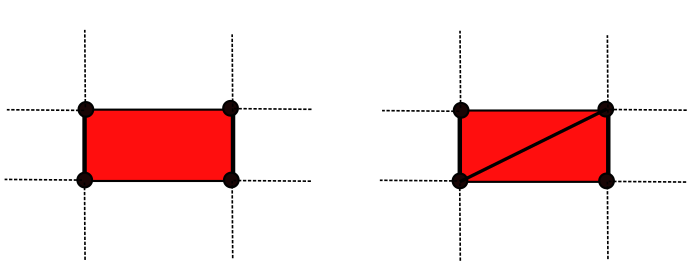
\includegraphics[width=0.6\columnwidth]{rectangulation}
					\caption{Turning a rectangular decomposition region into a triangulation by adding a diagonal}
					\label{fig:rectangulation}
				\end{figure}
		
			\noindent Observe that the total number of vertices for the rectangle does not change. For each face we had we add one extra edge and the the total number of faces doubles. This is summarized by the following maps. 
				\begin{equation*}
					\begin{cases}
						V \to V \\ 
						E \to E + F \\ 
						F \to 2F 
					\end{cases}
				\end{equation*}
			\noindent Thus we can easily verify our new Euler characteristic $\chi'(S)$. 
				\begin{equation*}
					\chi'(S) = V'-E'+F' = V-(E+F)+2F = V-E+F = \chi(S)
				\end{equation*}
			\noindent and so we see that the Euler characteristic is not impacted by this action. 
		
		\end{proof}
		
		\begin{proof}[(b)]
			\begin{figure}[!hbt]
				\centering
				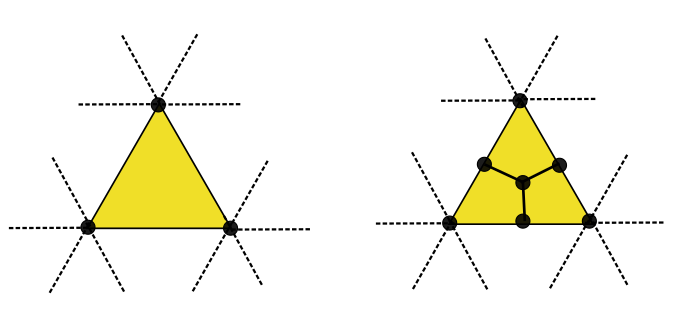
\includegraphics[width=0.5\columnwidth]{triangulation}
				\caption{Creating rectangles in a triangulation}
				\label{fig:triangulation} 
			\end{figure}
			
			Observe that this process adds one vertex for every face as well as one vertex for every preexisting edge. We add three edges for every previous face and every previous edge gets turned into two edges. The total number of faces triples. This is summarized by the following mappings 
				\begin{equation*}
					\begin{cases}
						V \to V+E+F \\ 
						E \to 2E + 3F \\ 
						F \to 3F 
					\end{cases}
				\end{equation*}
			\noindent Thus we can verify that the Euler characteristic does not change. 
				\begin{equation*}
					\chi'(S) = V'-E'+F' = (V+E+F)-(2E+3F)+(3F) = V-E+F = \chi(S)
				\end{equation*}
		\end{proof}
		
		\begin{proof}[(c)]
			Consider a generalized decomposition by N-gons. I will demonstrate a procedure that preserves the Euler characteristic and leads to a triangulation. First, choose one vertex v. Connect v to the v+2 vertex two places to the left with a line. This action maintains the Euler characteristic because the number of vertices does not change, we add one edge for every face, and the total number of faces doubles. i.e. 
				\begin{equation*}
					\begin{cases}
						V \to V \\ 
						E \to E + F \\ 
						F \to 2F
					\end{cases}
				\end{equation*}	
			so that the characteristic becomes 
				\begin{equation*}
					\chi'(S) = V'-E'+F' = V-(E+F)+2F = V-E+F = \chi(S)
				\end{equation*}
				
				
			\begin{figure}[!hbt]
				\centering
				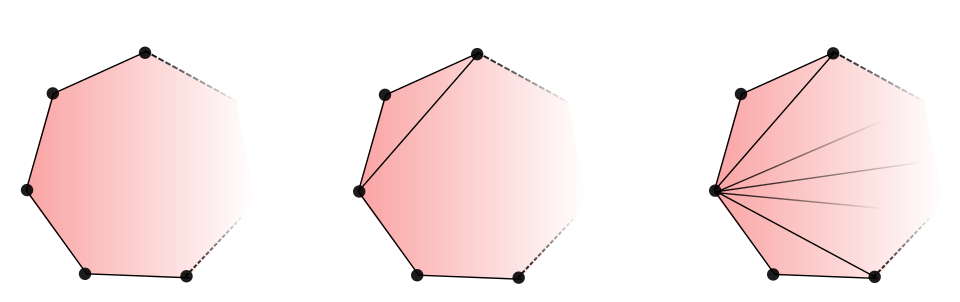
\includegraphics[width=0.5\columnwidth]{ngon}
				\caption{Turning an n-gon into n-2 triangles}
				\label{fig:ngon} 
			\end{figure}
			
			\noindent After such a move is made the result is a triangle and a (n-1)-gon. By induction we can repeat this process until the original vertex v has been connected to every other vertex with by an edge so that we obtain (n-2) triangles for every original polygon. Notice that part (a) was just the application of this process to a rectangular decomposition (4-gons).\\ 
			
			\noindent Because all we are doing is repeating the same move which itself preserves the Euler characteristic, we can always carry out this process until we have a true triangulation without changing $\chi(S)$. 
		\end{proof}
		
		
\end{document}





















































